%% ------------------------------------------------------------------------- %%
\chapter{Final Conclusions}
\label{cap:conclusoes}

\section{BEM Efficiency as a Computational Tool}

We can discuss the efficiency of BEM as a computational tool from the obtained results.

Since all costly routines of BEM can be paralellized, its implementation can take advantage 
of multicore machines and GPUs to reduce the time required in simulations.

Since the GeForce GTX 980 provided stunning resuts in \texttt{Venus}, a home computer paired 
with such GPU can execute the simulation faster without investing into a more costly server. 
Similar results were published in WSCAD-WIC conference, earning second place in the best paper 
category \citep{belinassi:2017}.


When compared to the original program, the total time elapsed in the simulation was reduced to a 
margin that is feasible for bigger mesh numbers such as the 14400 sample, as shown in
Figure $\ref{fig:total_brucutuiv}$. It is possible to archive even more speedups if a load balancer 
is implemented in a way that it can use both CPU and GPU in parallel.

If there is a major concern about errors in the simulation, perhaps caution is required when offloading 
the task to the GPU, as the mainly graphic on Figure $\ref{fig:ghmatecd_brucutuiv_error}$ indicates.

\begin{figure}[ht]
\centering
\textbf{Total elapsed time in \texttt{BrucutuIV}}\par\medskip
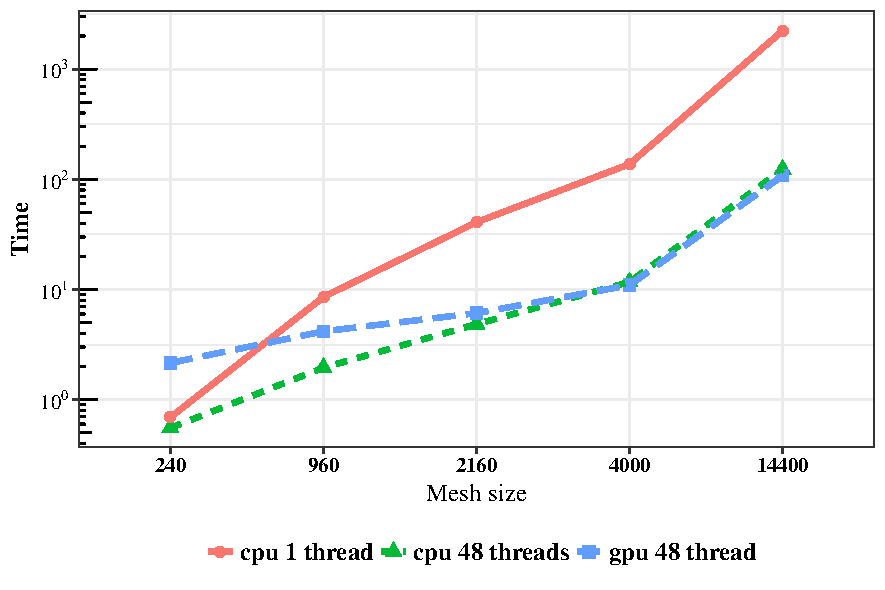
\includegraphics[scale=1]{total_brucutuiv.pdf}
\caption{Total elapsed time in \texttt{BrucutuIV}. One data per sample}
\label{fig:total_brucutuiv}
\end{figure}

As a final conclusion, the program can now be used to simulate cases where the original couldn't 
because of time constraints or unecessary memory usage. It also has no issues running in modern 
Linux distribuitions once all project dependencies are installed.

\section{As a Programmer}

Adding features regarding to a technology that did not exist in the time period of the program's 
development was a challenge at first mainly because of sparse support for the original language nowdays. 
Sure, calling C from Fortran in the way we presented enabled the current solution, 
but what if it couldn't be done in that way? That could be the case for even older systems.

Also, implementing numeric algorithms is no easy task because minor mistakes on a variable cause an 
absurd impact on results, but without crashing the program. Using automated tests to isolate the 
faulty routine is determinant for solving the problem because such incorrect results propagate to 
subsequent routines, causing the problem's source to be lost. Once such routine is detected, GDB 
is useful to determine what variable is the cause of such undesired behaviour. Tests are important 
and must not be underestimated.

As for the GPU development, testing an code is painful as we are unable to run \texttt{X11} and \texttt{cuda-gdb} 
in the same GPU  simultaneously. Additionaly, sometimes a \texttt{SEGFAULT} in a CUDA kernel caused the computer 
to hang, requiring a complete reboot of the machine. 
One last complain is that it is not possible to allocate multiple arrays in CUDA's shared memory dynamically, 
requiring pointer magic to allocate multiple arrays into a single array. All these points require improvements. 

\section{Future Works}

The presented implementation can still be improved. A load balancer can be developed for 
distribuiting workload between CPU and GPU for constructing the $H$ and $G$ matrices from 
\texttt{Ghmatece} and \texttt{Ghmatecd} routines for better speedups.  

The linear system solving routine can run quickier simply by keeping the $H$ 
matrix in GPU memory. This is not already implemented due to the structure of the actual 
program, a refactoration is necessary.

A better parallel strategy for reducing the matrix (as illustrated by the function \newline 
\texttt{SumAllMatricesInBuffer} of Algorithms $\ref{ghmatecd_new}$ and $\ref{ghmatecd_new2}$) is 
required for better speedups. This can lead to even better speedups.
